\chapter{Results}
\label{chap:results}
\section{Production prevision for a single turbine}
\label{sec:res_single}

The evaluation of the model for the simulation of a single plant with precise input data (see Sec. \ref{sub:metho_single}) was carried out on the HydroRaon power plant operated by the company Ercisol \cite{ercisol}. It was rebuilt on the site of an old run-of-the-river plant, dismantled fifteen years ago. This production site was chosen in our study for the availability of runoff data, plant parameters, and production data. However, its operation started recently (12\textsuperscript{th} of April 2017) and the first months of operation were a running in phase during which the plant underwent adjustments and did not operate to its full potential. \newline
Figure \ref{raon_map} shows the locations of the plant and the closest gauge station, with their parameters. Table \ref{prod_raon} gives the measured monthly production of the plant, as published by the company on their website, as well as the production simulated with the model, using the hourly runoff time series from the ``Banque Hydro'' \cite{eaufrance}. April's production was calculated starting on the 12\textsuperscript{th}, when the plant started operating. The hourly production is represented in Fig. \ref{prod_raon_curve}.

\begin{table}[H]
\footnotesize
 \centering
 \caption{Monthly production of the HydroRaon plant}
 \label{prod_raon}
 \begin{tabular}{l|c|c|c|}
  &Ercisol data \cite{ercisol}&Model output&\multirow{2}{*}{Difference}\\
  Month&Measured [MWh]&Simulated [MWh]&\\
  \hline
  April&37&63&+\unit[70]{\%}\\
  May&86&123&+\unit[43]{\%}\\
  June&66&100&+\unit[51]{\%}\\
  July&29&39&+\unit[34]{\%}\\
  August&17&13&-\unit[23]{\%}\\
 \end{tabular}
\end{table}

\begin{figure}[H]
\centering
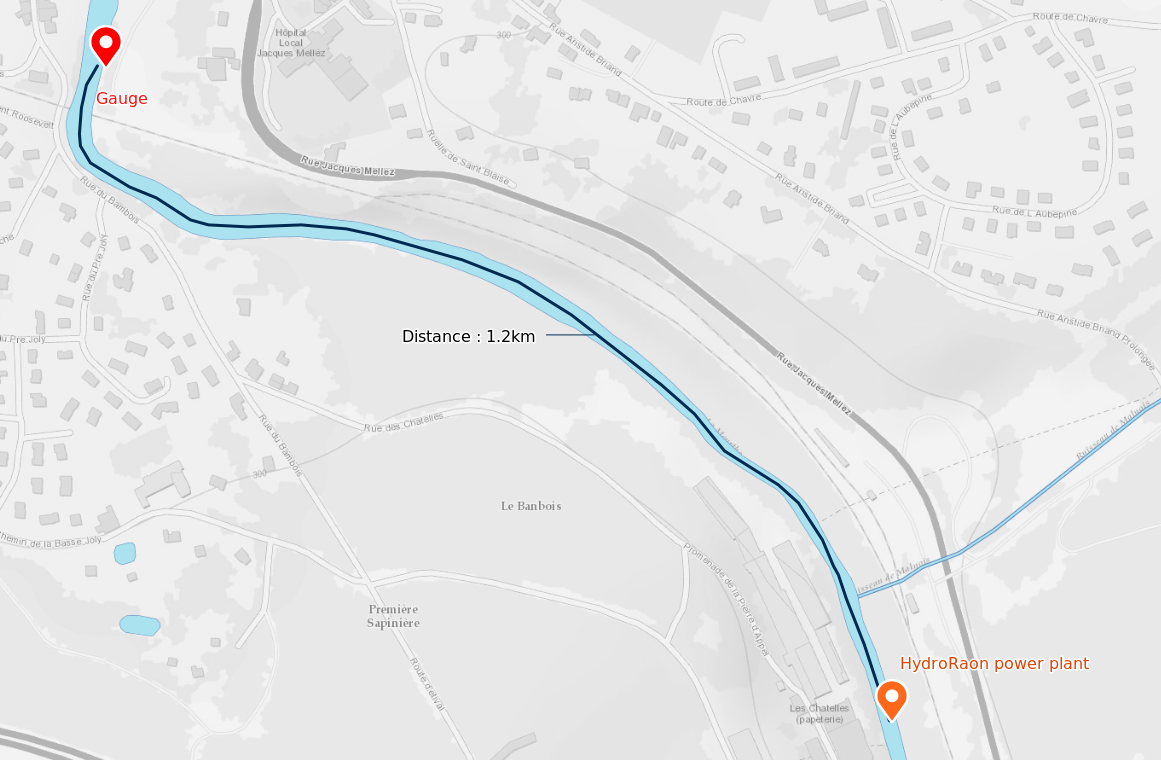
\includegraphics[width=14cm]{raon_map.png}
\caption{Sites and parameters of the HydroRaon plant and the Raon gauge station}
\label{raon_map}
\end{figure}

\begin{figure}[H]
\centering
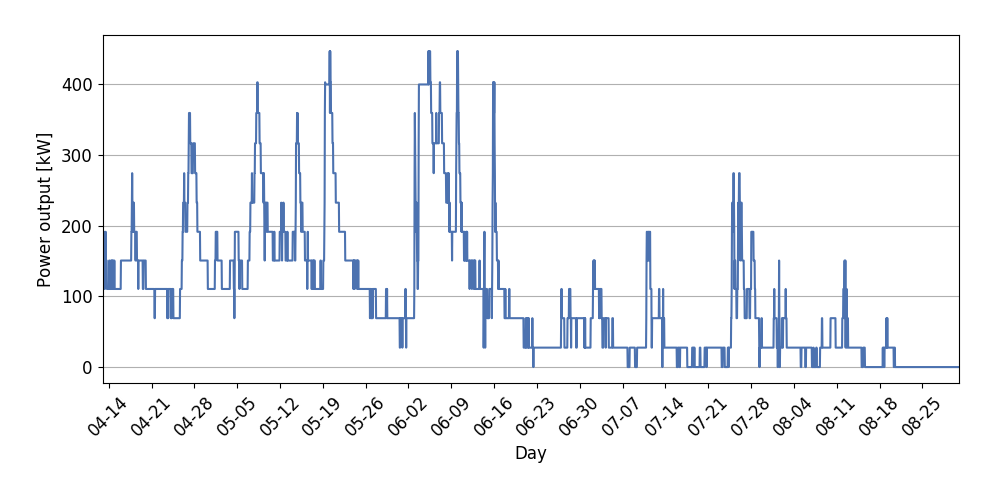
\includegraphics[width=15cm]{prod_raon_curve.png}
\caption{Simulated production of the HydroRaon plant}
\label{prod_raon_curve}
\end{figure}

From April to July the simulated production is significantly superior to the measured production of the plant. This is due to the fact that the plant had just started operating and was undergoing tests and adjustments. In August, the simulated production is under the measured production. These results will be discussed in Ch. \ref{chap:discussion}.

\section{Extrapolation of power plant data}
\label{sec:missing_data}
Section \ref{sub:metho_extra} lists plants for which both precise design parameters (nominal water flow, nominal head, number and type of turbines) and runoff data were available. The process of extrapolating missing data was tested for these plants. Their nominal power and number of turbines were fed to the model, and the results of the parameter extrapolation process was compared with the actual plant parameters. This process was done with measured and modelled runoffs as input. The results are given in Tab. \ref{tab_res_extra} which lists for each station the real and simulated nominal water flows, heads and turbine types. Simulation A is based on modelled runoffs while simulation B is based on measured runoffs. \newline
The results of the simulation based on modelled runoff data shows several values very far from reality, where a very low nominal water flow has been set, inducing an extremely high head. Figure \ref{map_mosel_watergap} shows that this happens for plants located in raster cells with a low mean runoff (<\unit[10]{m\textsuperscript{3}\textperiodcentered s\textsuperscript{-1}}), not representative of the Mosel. In Koblenz, where the Mosel meets the Rhine, the runoff of the cell is representative of the Rhine, which has a much higher water flow. Therefore, the nominal water flow for the plant in Koblenz, located on the Mosel, is higher than the real nominal water flow, and the head is smaller. Moreover, Sec. \ref{sub:assumptions} explains that the extrapolation process follows the steps of the design process of a run-of-the-river power plant. This design process is normally based on the study of runoff time series over several decades preceding the plant construction, while modelled time series available for this study covered only the years 2006 to 2009. \newline
This faulty assignment of the nominal head and nominal water flow leads to a erroneous assignment of the turbine type, since it is assigned based on the characteristic h\textsubscript{n}/\.V\textsubscript{n} diagram (Fig. \ref{charac_diag}). \newline
The results based on measured runoff data seem to provide more coherent results. However, if this process gives good results for large waterways with a steady flow and numerous gauge stations, it is bound to entail uncertainties when applied to plants on minor rivers: in this case, the extrapolation process can be done on runoff data from a much bigger river than the one the plant is actually on.\newline
Section \ref{sec:improv} shows that this extrapolation process has a big impact on the simulated production and prompts the need for a better adjustment of the runoff data to the plants, for the extrapolation process to be based on consistent data.


\begingroup
\renewcommand\arraystretch{0.8}
\begin{longtable}{|c|c|c|c|c|}
 \caption{Results of the parameter extrapolation process}
 \label{tab_res_extra}\\
 \hline
  \textbf{Plant}&\textbf{Parameter}&\textbf{Real}&\textbf{Simulation A}&\textbf{Simulation B}\\
  \hline
  \endhead
  \hline
  \endfoot
  \multirow{3}{*}{HydroRaon}&\.V\textsubscript{n}&12&11.1&18.4\\
  &h\textsubscript{n}&4.23&4.29&2.60\\
  &Turbine type&Kaplan&Kaplan&Kaplan\\
  \hline
  \multirow{3}{*}{Koblenz}&\.V\textsubscript{n}&380&2371&438\\
  &h\textsubscript{n}&5.3&0.8&4.36\\
  &Turbine type&Kaplan&dummy&Kaplan\\
  \hline
  \multirow{3}{*}{Lehmen}&\.V\textsubscript{n}&400&360&438\\
  &h\textsubscript{n}&7.5&6.6&5.44\\
  &Turbine type&Kaplan&Kaplan&Kaplan\\
  \hline
  \multirow{3}{*}{Müden}&\.V\textsubscript{n}&400&360&438\\
  &h\textsubscript{n}&6.5&5.4&4.46\\
  &Turbine type&Kaplan&Kaplan&Kaplan\\
  \hline
  \multirow{3}{*}{Fankel}&\.V\textsubscript{n}&400&359&438\\
  &h\textsubscript{n}&7&5.4&4.46\\
  &Turbine type&Kaplan&Kaplan&Kaplan\\
  \hline
  \multirow{3}{*}{Neef}&\.V\textsubscript{n}&400&0.4&438\\
  &h\textsubscript{n}&7&5538&4.46\\
  &Turbine type&Kaplan&dummy&Kaplan\\
  \hline
  \multirow{3}{*}{Enkirch}&\.V\textsubscript{n}&400&1.2&438\\
  &h\textsubscript{n}&7.5&1808&5\\
  &Turbine type&Kaplan&Kaplan&Kaplan\\
  \hline
  \multirow{3}{*}{Zeltingen}&\.V\textsubscript{n}&400&350&438\\
  &h\textsubscript{n}&6&4.6&3.7\\
  &Turbine type&Kaplan&Kaplan&Kaplan\\
  \hline
  \multirow{3}{*}{Wintrich}&\.V\textsubscript{n}&400&0.3&381\\
  &h\textsubscript{n}&7.5&8192&6.25\\
  &Turbine type&Kaplan&dummy&Kaplan\\
  \hline
  \multirow{3}{*}{Detzem}&\.V\textsubscript{n}&400&13.3&381\\
  &h\textsubscript{n}&9&30.6&7.5\\
  &Turbine type&Kaplan&dummy&Kaplan\\
  \hline
  \multirow{3}{*}{Trier}&\.V\textsubscript{n}&400&0.6&381\\
  &h\textsubscript{n}&7.25&3768&5.9\\
  &Turbine type&Kaplan&dummy&Kaplan\\
  \hline
  \multirow{3}{*}{Grevenmacher}&\.V\textsubscript{n}&165&5.2&381\\
  &h\textsubscript{n}&6.25&180&2.4\\
  &Turbine type&Kaplan&Francis&Kaplan\\
  \hline
  \multirow{3}{*}{Paltzem}&\.V\textsubscript{n}&150&125&214\\
  &h\textsubscript{n}&4&4.3&2.5\\
  &Turbine type&Kaplan&Kaplan&Kaplan\\
\end{longtable}
\endgroup

\begin{figure}[H]
\centering
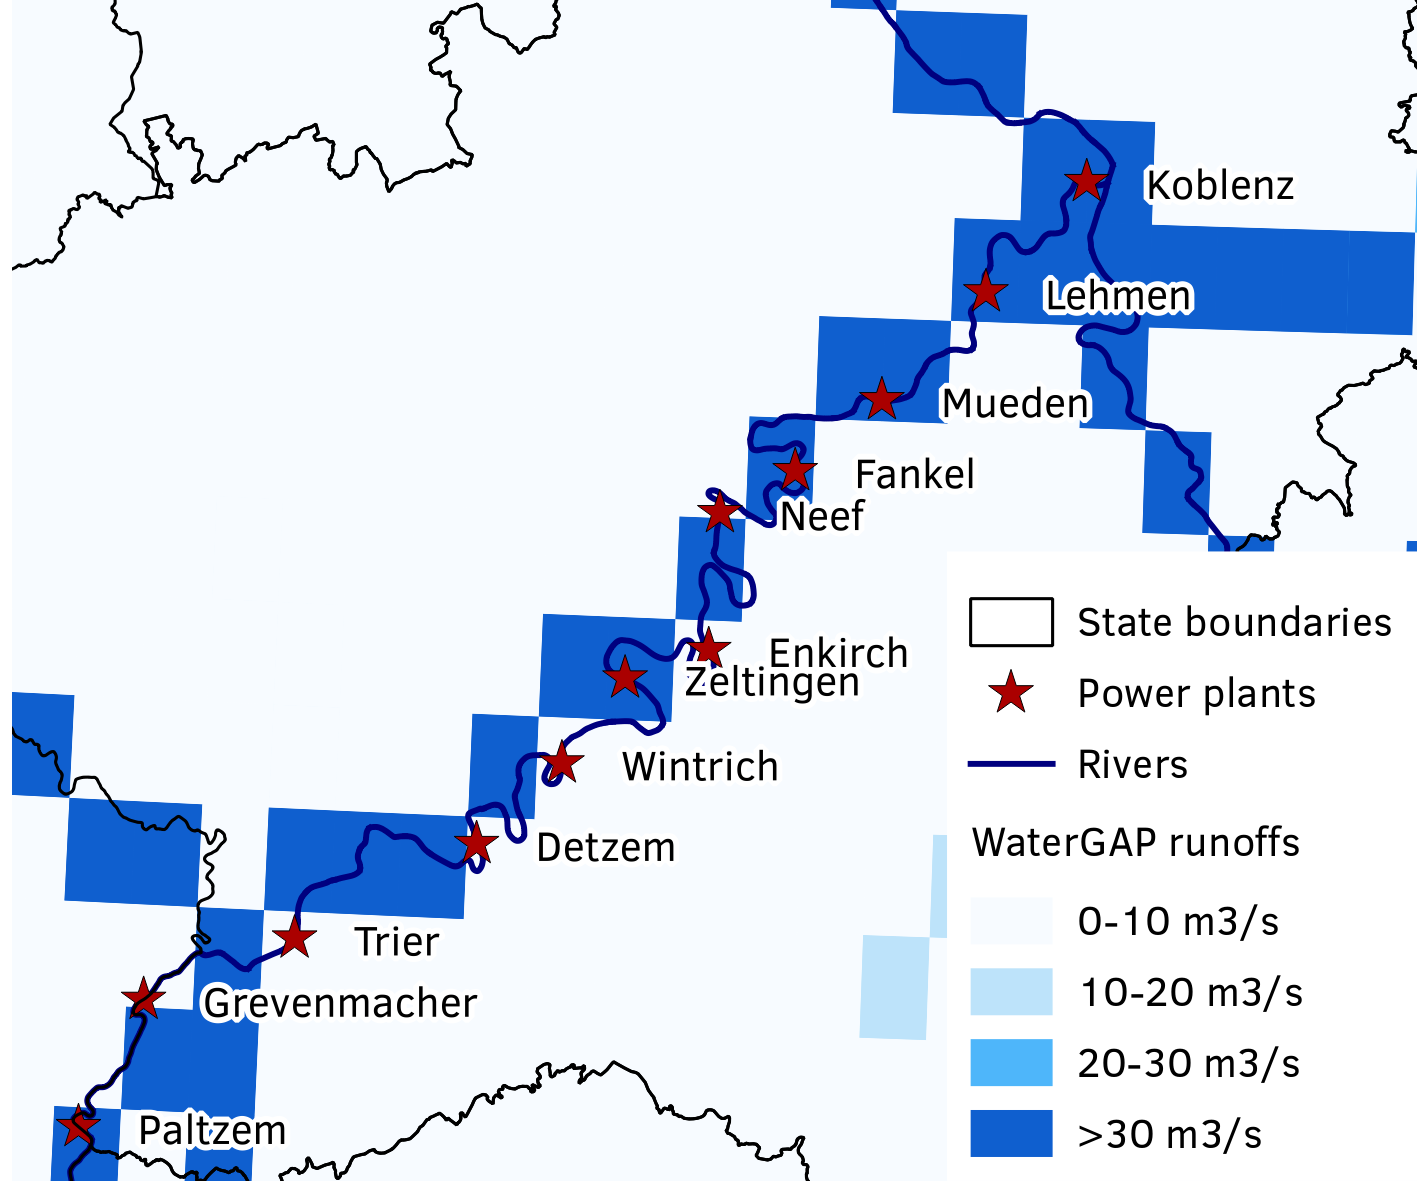
\includegraphics[width=10cm]{map_mosel_watergap.png}
\caption{Power plants of the Mosel with average modelled runoffs}
\label{map_mosel_watergap}
\end{figure}

\section{Production prevision for a region}
\label{sec:res_th}

Sections \ref{sec:db_hydroelec} and \ref{sub:metho_sw} showed the problems inherent to comparing the results of a state-wide simulation based on the OpenEnergy Database with publicly available production data (from the Agentur für Erneuerbare Energien - AEE). Firstly, the AEE aggregates data from run-of-the-river plants, reservoir plants, as well as some pumped storage plants instead of differentiating them like the Open Power System Data. Secondly, the OPSD registers, in terms of number of plants and installed capacity, are not consistent with the AEE aggregated data, and the inconsistencies cannot be explained by the precedent remark alone. \newline
Section \ref{sub:metho_sw} justified the choice of running the state-wide simulation on the federal state of Thuringia, and the results are presented here. \newline
The OPSD lists 205 run-of-the-river plants for Thuringia, displayed in Fig. \ref{map_th} along with the 18 used gauge stations, the average values of modelled runoff, and the river network.

\begin{figure}[H]
\centering
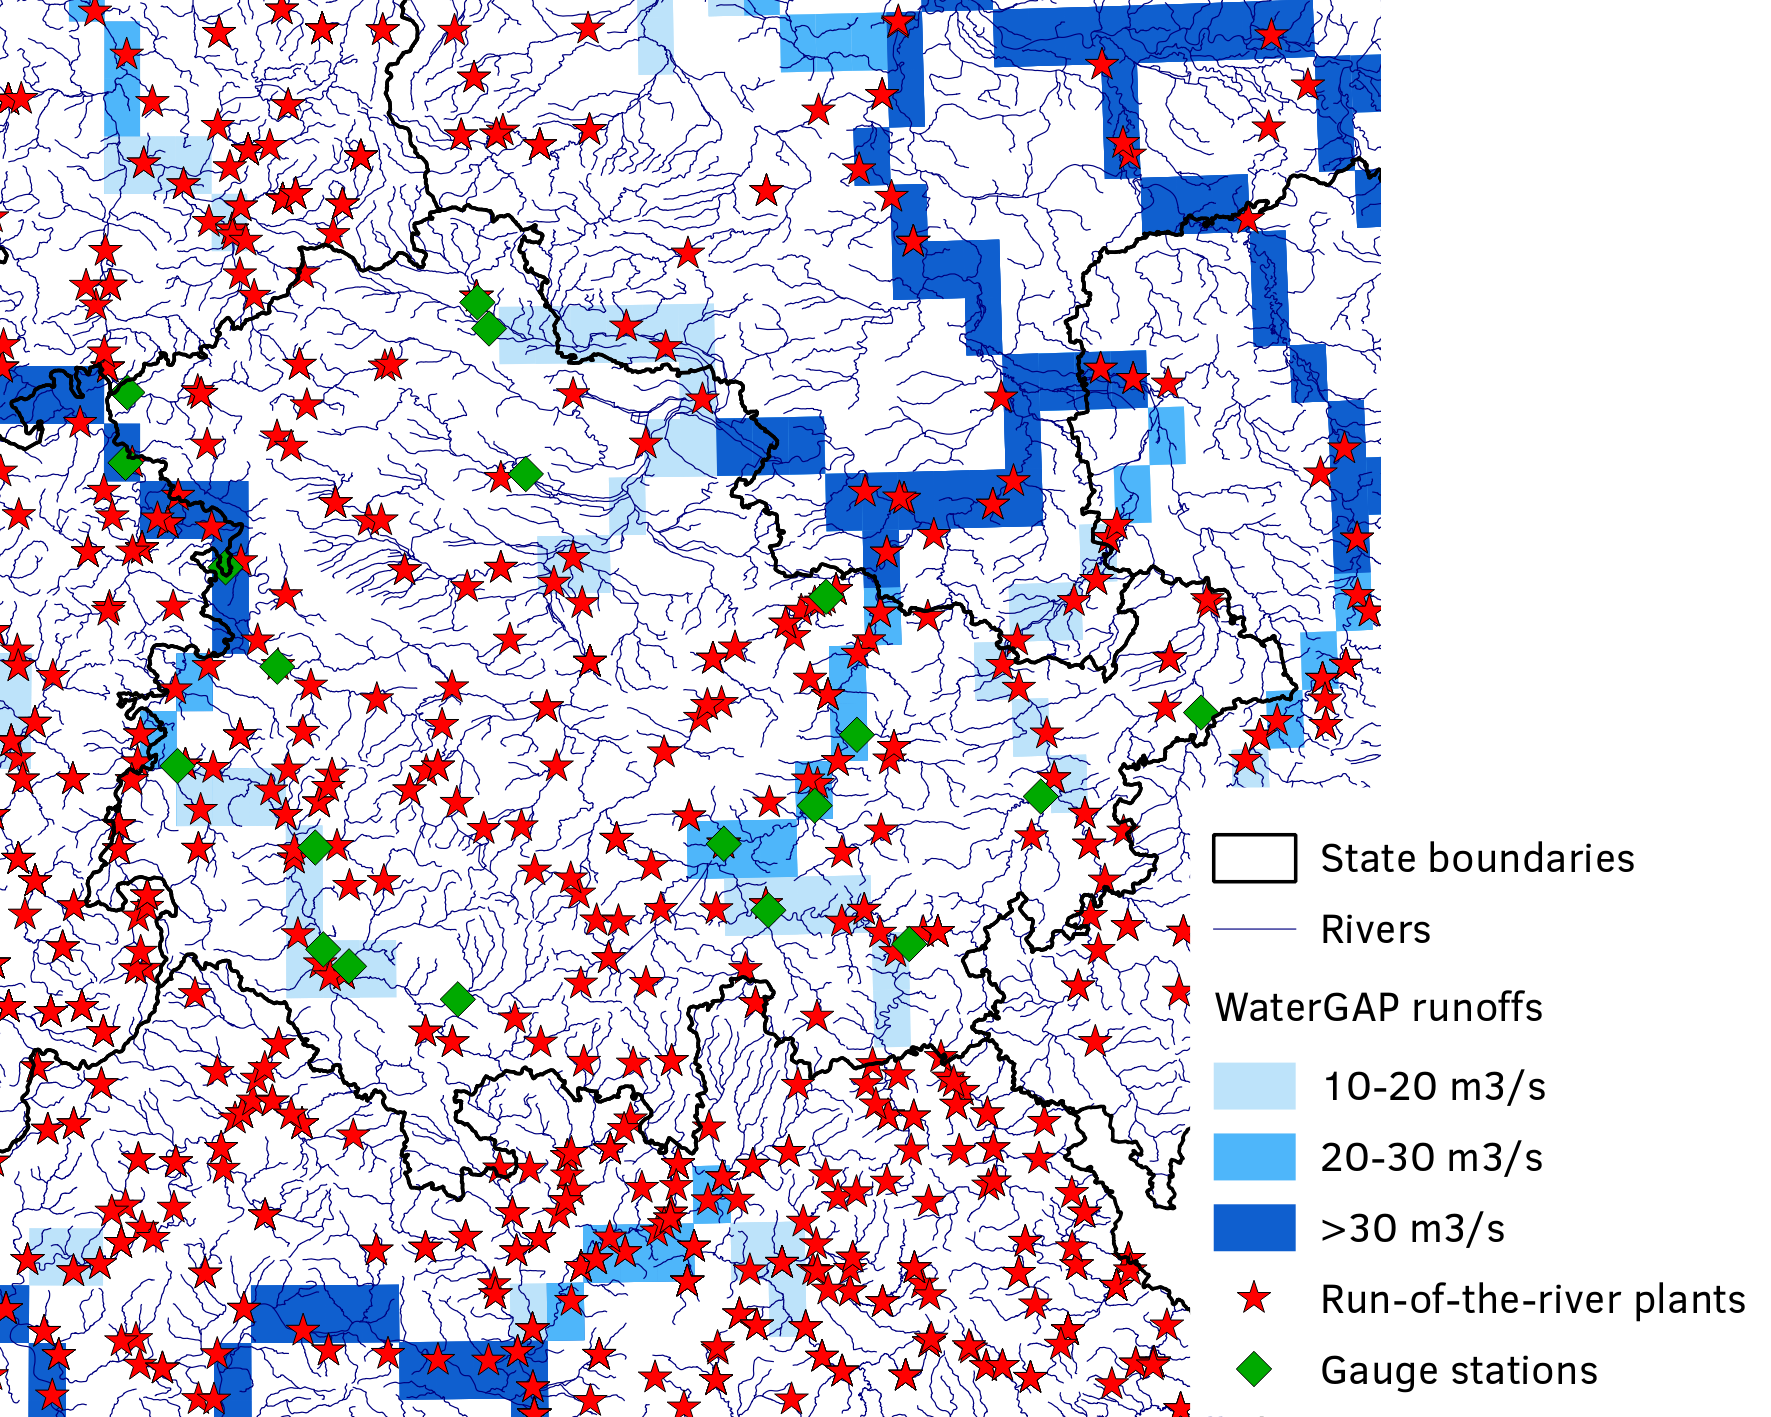
\includegraphics[width=13cm]{map_th.png}
\caption{Run-of-the-river plants, gauge stations, river and modelled runoff in Thuringia}
\label{map_th}
\end{figure}

\begin{table}[H]
\footnotesize
 \centering
 \caption{Yearly production of Thuringia: measured and simulated data}
 \label{res_th}
 \begin{tabular}{|l|ccc|}
 \hline
  &\multicolumn{3}{c|}{Yearly production in MWh}\\
  Year&Published by AEE&Simulated from modelled runoffs&Simulated from measured runoff\\
  \hline \hline
  \multirow{2}{*}{2005}&\multirow{2}{*}{180}&119&-\\
  &&-\unit[34]{\%}&-\\
  \hline
  \multirow{2}{*}{2006}&\multirow{2}{*}{163}&105&112\\
  &&-\unit[36]{\%}&-\unit[31]{\%}\\
  \hline
  \multirow{2}{*}{2007}&\multirow{2}{*}{322}&175&162\\
  &&-\unit[46]{\%}&-\unit[50]{\%}\\
  \hline
  \multirow{2}{*}{2008}&\multirow{2}{*}{248}&131&187\\
  &&-\unit[47]{\%}&-\unit[25]{\%}\\
  \hline
  \multirow{2}{*}{2009}&\multirow{2}{*}{200}&-&130\\
  &&-&-\unit[35]{\%}\\
  \hline
 \end{tabular}
\end{table}

Two state-wide simulations were made: one based on modelled runoff and one based on measured runoff. The data was preprocessed following the guidelines of Sec. \ref{sub:pp_reg}: the location of the plants was refined, placing them on the course of the nearest river, and they were assigned a gauge station (in the case of measured runoff) or raster cell (in the case of modelled runoff). The yearly productions are given in Tab. \ref{res_th} and compared with the AEE values, and the productions of each plant are displayed in Fig. \ref{prod_th_map}.

\begin{figure}[H]
\centering
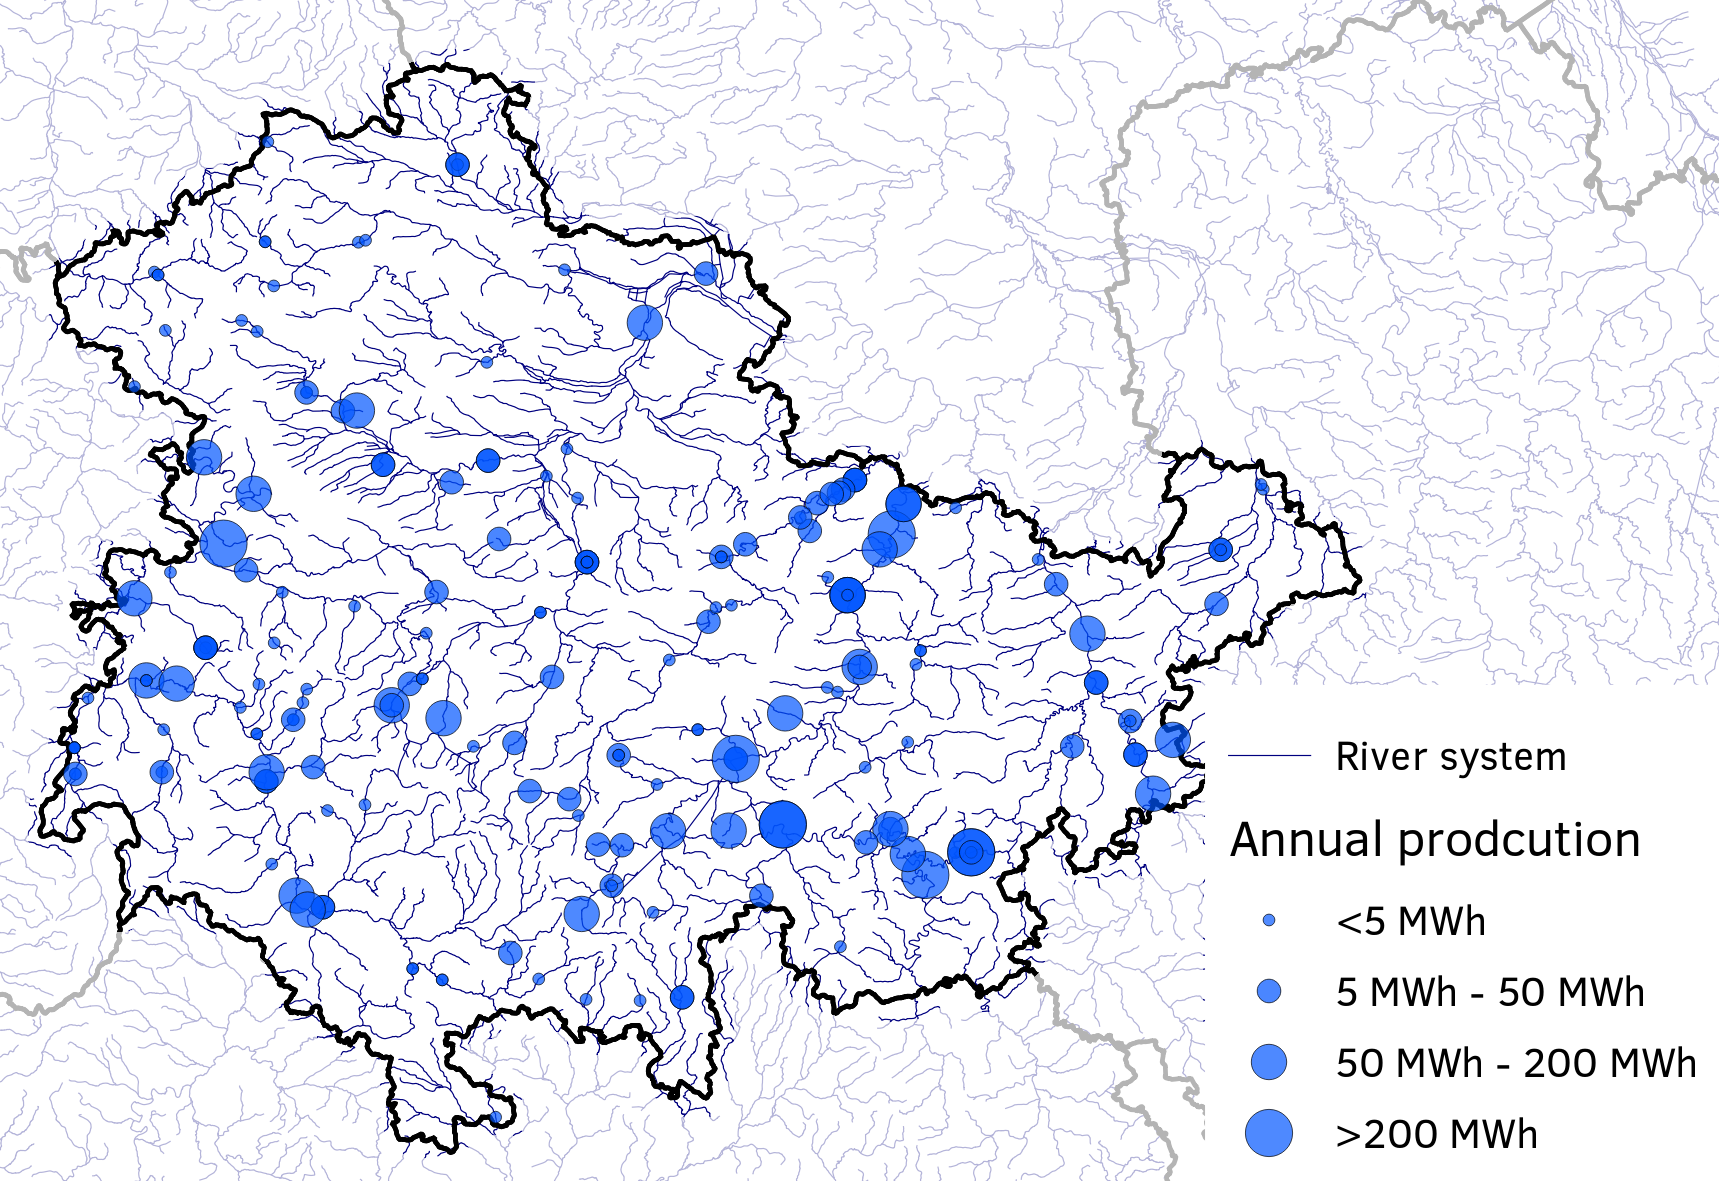
\includegraphics[width=13cm]{prod_th_map.png}
\caption{Simulated production of run-of-the-river plants in Thuringia, based on modelled runoffs, year 2009}
\label{prod_th_map}
\end{figure}
 
The production is significantly underestimated by both simulation processes, and a more advanced analysis with precise data about plants would be needed to assess if the difference is due to the inconsistencies between the AEE and OPSD data sets, and if not, which parts of the simulation process causes this difference. Some ideas are given in Sec. \ref{sec:improv}.